\documentclass{standalone}
\usepackage{tikz}
\usetikzlibrary{patterns, positioning}

\begin{document}
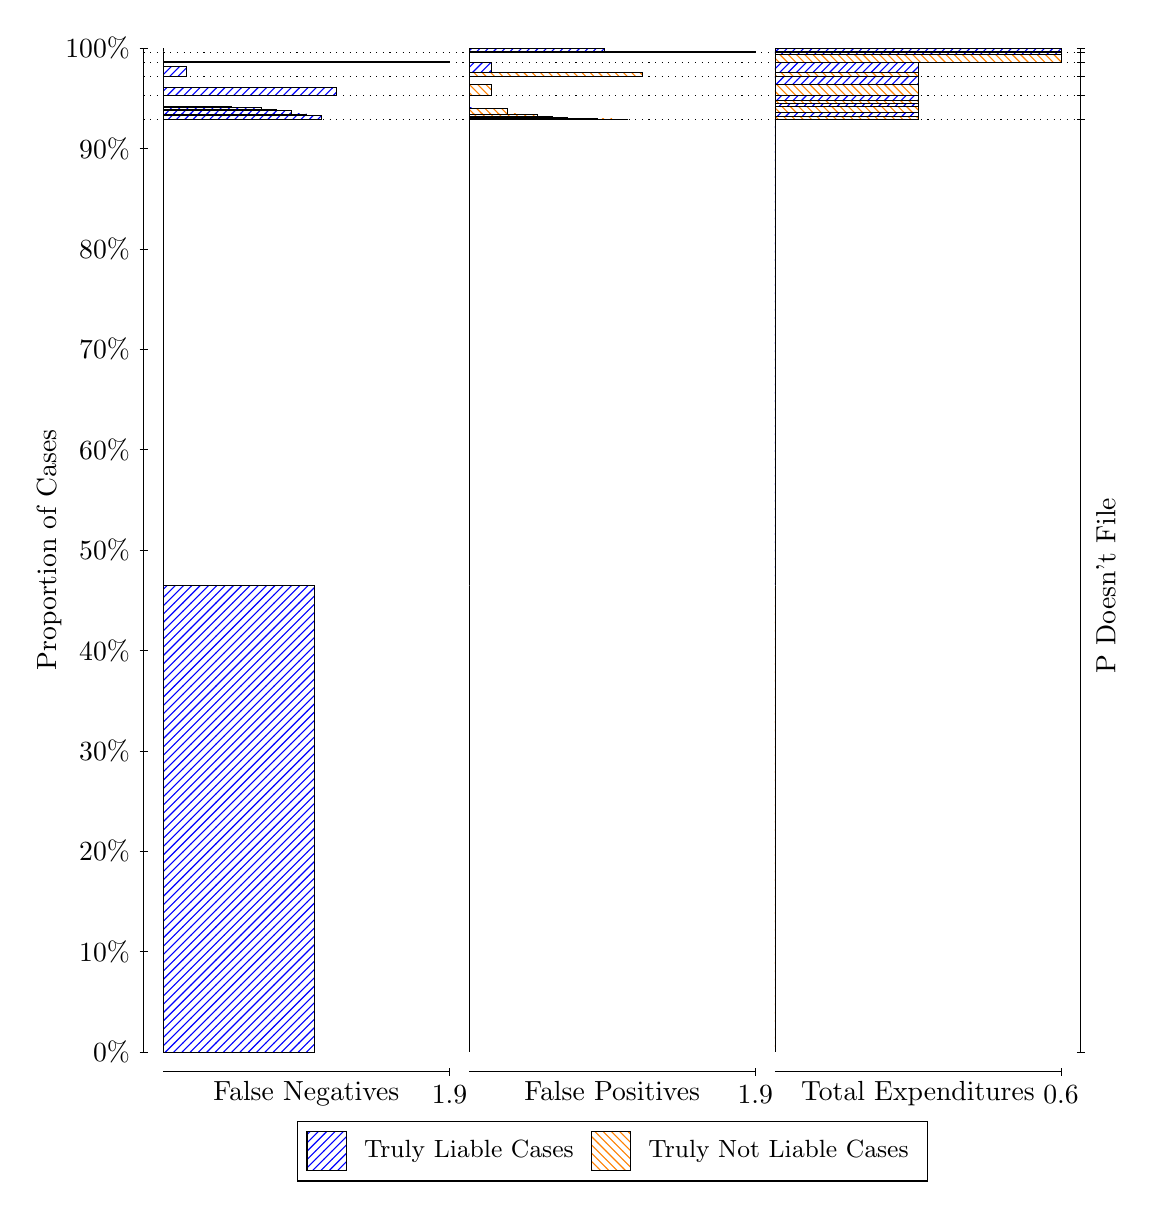
\begin{tikzpicture}
\draw[black, very thin] (1.5,1.75) -- (1.5,14.5);
\node[rotate=90, anchor=center] at (0.3, 8.125) {Proportion of Cases};
\draw[black, very thin] (1.45,1.75) -- (1.55,1.75);
\node[anchor=east] at (1.45, 1.75) {0\%};
\draw[black, very thin] (1.45,3.025) -- (1.55,3.025);
\node[anchor=east] at (1.45, 3.025) {10\%};
\draw[black, very thin] (1.45,4.3) -- (1.55,4.3);
\node[anchor=east] at (1.45, 4.3) {20\%};
\draw[black, very thin] (1.45,5.575) -- (1.55,5.575);
\node[anchor=east] at (1.45, 5.575) {30\%};
\draw[black, very thin] (1.45,6.85) -- (1.55,6.85);
\node[anchor=east] at (1.45, 6.85) {40\%};
\draw[black, very thin] (1.45,8.125) -- (1.55,8.125);
\node[anchor=east] at (1.45, 8.125) {50\%};
\draw[black, very thin] (1.45,9.4) -- (1.55,9.4);
\node[anchor=east] at (1.45, 9.4) {60\%};
\draw[black, very thin] (1.45,10.675) -- (1.55,10.675);
\node[anchor=east] at (1.45, 10.675) {70\%};
\draw[black, very thin] (1.45,11.95) -- (1.55,11.95);
\node[anchor=east] at (1.45, 11.95) {80\%};
\draw[black, very thin] (1.45,13.225) -- (1.55,13.225);
\node[anchor=east] at (1.45, 13.225) {90\%};
\draw[black, very thin] (1.45,14.5) -- (1.55,14.5);
\node[anchor=east] at (1.45, 14.5) {100\%};

\draw[black, very thin] (13.4,1.75) -- (13.4,14.5);
\draw[black, very thin] (13.35,1.75) -- (13.45,1.75);
\node[anchor=west] at (13.35, 1.75) {};
\draw[black, very thin] (13.35,13.596) -- (13.45,13.596);
\node[anchor=west] at (13.35, 13.596) {};
\draw[black, very thin] (13.35,13.901) -- (13.45,13.901);
\node[anchor=west] at (13.35, 13.901) {};
\draw[black, very thin] (13.35,14.142) -- (13.45,14.142);
\node[anchor=west] at (13.35, 14.142) {};
\draw[black, very thin] (13.35,14.315) -- (13.45,14.315);
\node[anchor=west] at (13.35, 14.315) {};
\draw[black, very thin] (13.35,14.44) -- (13.45,14.44);
\node[anchor=west] at (13.35, 14.44) {};
\draw[black, very thin] (13.35,14.5) -- (13.45,14.5);
\node[anchor=west] at (13.35, 14.5) {};

\draw[black, very thin, pattern color=blue, pattern=north east lines] (1.75,1.75) rectangle (3.6623,7.6727);
\draw[black, very thin, pattern color=orange, pattern=north west lines] (1.75,7.6727) rectangle (1.75,13.596);
\draw[black, very thin, pattern color=blue, pattern=north east lines] (1.75,13.596) rectangle (3.7579,13.642);
\draw[black, very thin, pattern color=blue, pattern=north east lines] (1.75,13.642) rectangle (3.5667,13.665);
\draw[black, very thin, pattern color=blue, pattern=north east lines] (1.75,13.665) rectangle (3.3754,13.705);
\draw[black, very thin, pattern color=blue, pattern=north east lines] (1.75,13.705) rectangle (3.1842,13.725);
\draw[black, very thin, pattern color=blue, pattern=north east lines] (1.75,13.725) rectangle (2.993,13.745);
\draw[black, very thin, pattern color=blue, pattern=north east lines] (1.75,13.745) rectangle (2.8018,13.75);
\draw[black, very thin, pattern color=blue, pattern=north east lines] (1.75,13.75) rectangle (2.6105,13.754);
\draw[black, very thin, pattern color=blue, pattern=north east lines] (1.75,13.754) rectangle (2.4193,13.756);
\draw[black, very thin, pattern color=blue, pattern=north east lines] (1.75,13.756) rectangle (2.2281,13.758);
\draw[black, very thin, pattern color=orange, pattern=north west lines] (1.75,13.758) rectangle (1.75,13.901);
\draw[black, very thin, pattern color=blue, pattern=north east lines] (1.75,13.901) rectangle (3.9491,14.004);
\draw[black, very thin, pattern color=orange, pattern=north west lines] (1.75,14.004) rectangle (1.75,14.142);
\draw[black, very thin, pattern color=blue, pattern=north east lines] (1.75,14.142) rectangle (2.0368,14.268);
\draw[black, very thin, pattern color=orange, pattern=north west lines] (1.75,14.268) rectangle (1.75,14.315);
\draw[black, very thin, pattern color=blue, pattern=north east lines] (1.75,14.315) rectangle (5.3833,14.334);
\draw[black, very thin, pattern color=orange, pattern=north west lines] (1.75,14.334) rectangle (1.75,14.44);
\draw[black, very thin, pattern color=orange, pattern=north west lines] (1.75,14.44) rectangle (1.75,14.459);
\draw[black, very thin, pattern color=blue, pattern=north east lines] (1.75,14.459) rectangle (1.75,14.5);
\draw[black, very thin, pattern color=orange, pattern=north west lines] (5.6333,1.75) rectangle (5.6333,7.6729);
\draw[black, very thin, pattern color=blue, pattern=north east lines] (5.6333,7.6729) rectangle (5.6333,13.596);
\draw[black, very thin, pattern color=orange, pattern=north west lines] (5.6333,13.596) rectangle (7.6412,13.598);
\draw[black, very thin, pattern color=orange, pattern=north west lines] (5.6333,13.598) rectangle (7.45,13.6);
\draw[black, very thin, pattern color=orange, pattern=north west lines] (5.6333,13.6) rectangle (7.2588,13.604);
\draw[black, very thin, pattern color=orange, pattern=north west lines] (5.6333,13.604) rectangle (7.0675,13.608);
\draw[black, very thin, pattern color=orange, pattern=north west lines] (5.6333,13.608) rectangle (6.8763,13.621);
\draw[black, very thin, pattern color=orange, pattern=north west lines] (5.6333,13.621) rectangle (6.6851,13.63);
\draw[black, very thin, pattern color=orange, pattern=north west lines] (5.6333,13.63) rectangle (6.6851,13.632);
\draw[black, very thin, pattern color=orange, pattern=north west lines] (5.6333,13.632) rectangle (6.4939,13.653);
\draw[black, very thin, pattern color=orange, pattern=north west lines] (5.6333,13.653) rectangle (6.3026,13.665);
\draw[black, very thin, pattern color=orange, pattern=north west lines] (5.6333,13.665) rectangle (6.1114,13.738);
\draw[black, very thin, pattern color=blue, pattern=north east lines] (5.6333,13.738) rectangle (5.7289,13.74);
\draw[black, very thin, pattern color=blue, pattern=north east lines] (5.6333,13.74) rectangle (5.6333,13.901);
\draw[black, very thin, pattern color=orange, pattern=north west lines] (5.6333,13.901) rectangle (5.9202,14.039);
\draw[black, very thin, pattern color=blue, pattern=north east lines] (5.6333,14.039) rectangle (5.6333,14.142);
\draw[black, very thin, pattern color=orange, pattern=north west lines] (5.6333,14.142) rectangle (7.8325,14.189);
\draw[black, very thin, pattern color=blue, pattern=north east lines] (5.6333,14.189) rectangle (5.9202,14.315);
\draw[black, very thin, pattern color=orange, pattern=north west lines] (5.6333,14.315) rectangle (5.6333,14.421);
\draw[black, very thin, pattern color=blue, pattern=north east lines] (5.6333,14.421) rectangle (5.6333,14.44);
\draw[black, very thin, pattern color=orange, pattern=north west lines] (5.6333,14.44) rectangle (9.2667,14.459);
\draw[black, very thin, pattern color=blue, pattern=north east lines] (5.6333,14.459) rectangle (7.3544,14.5);
\draw[black, very thin, pattern color=orange, pattern=north west lines] (9.5167,1.75) rectangle (9.5167,7.6729);
\draw[black, very thin, pattern color=blue, pattern=north east lines] (9.5167,7.6729) rectangle (9.5167,13.596);
\draw[black, very thin, pattern color=orange, pattern=north west lines] (9.5167,13.596) rectangle (11.333,13.63);
\draw[black, very thin, pattern color=blue, pattern=north east lines] (9.5167,13.63) rectangle (11.333,13.681);
\draw[black, very thin, pattern color=orange, pattern=north west lines] (9.5167,13.681) rectangle (11.333,13.754);
\draw[black, very thin, pattern color=blue, pattern=north east lines] (9.5167,13.754) rectangle (11.333,13.8);
\draw[black, very thin, pattern color=orange, pattern=north west lines] (9.5167,13.8) rectangle (11.333,13.835);
\draw[black, very thin, pattern color=blue, pattern=north east lines] (9.5167,13.835) rectangle (11.333,13.901);
\draw[black, very thin, pattern color=orange, pattern=north west lines] (9.5167,13.901) rectangle (11.333,14.039);
\draw[black, very thin, pattern color=blue, pattern=north east lines] (9.5167,14.039) rectangle (11.333,14.142);
\draw[black, very thin, pattern color=orange, pattern=north west lines] (9.5167,14.142) rectangle (11.333,14.189);
\draw[black, very thin, pattern color=blue, pattern=north east lines] (9.5167,14.189) rectangle (11.333,14.315);
\draw[black, very thin, pattern color=orange, pattern=north west lines] (9.5167,14.315) rectangle (13.15,14.421);
\draw[black, very thin, pattern color=blue, pattern=north east lines] (9.5167,14.421) rectangle (13.15,14.44);
\draw[black, very thin, pattern color=orange, pattern=north west lines] (9.5167,14.44) rectangle (13.15,14.459);
\draw[black, very thin, pattern color=blue, pattern=north east lines] (9.5167,14.459) rectangle (13.15,14.5);
\draw[black, dotted] (1.5,13.596) -- (13.4,13.596);
\draw[black, dotted] (1.5,13.901) -- (13.4,13.901);
\draw[black, dotted] (1.5,14.142) -- (13.4,14.142);
\draw[black, dotted] (1.5,14.315) -- (13.4,14.315);
\draw[black, dotted] (1.5,14.44) -- (13.4,14.44);
\draw[black, very thin] (1.75,1.5) -- (5.3833,1.5);
\node[anchor=north] at (3.5667, 1.5) {False Negatives};
\draw[black, very thin] (5.3833,1.45) -- (5.3833,1.55);
\node[anchor=north] at (5.3833, 1.45) {1.9};

\draw[black, very thin] (5.6333,1.5) -- (9.2667,1.5);
\node[anchor=north] at (7.45, 1.5) {False Positives};
\draw[black, very thin] (9.2667,1.45) -- (9.2667,1.55);
\node[anchor=north] at (9.2667, 1.45) {1.9};

\draw[black, very thin] (9.5167,1.5) -- (13.15,1.5);
\node[anchor=north] at (11.333, 1.5) {Total Expenditures};
\draw[black, very thin] (13.15,1.45) -- (13.15,1.55);
\node[anchor=north] at (13.15, 1.45) {0.6};

\node[black, centered, rotate=90] at (13.72, 7.6728) {P Doesn't File};






\draw (7.449999999999999,1.5) node[draw=none] (baseCoordinate) {};
\begin{scope}[align=center]
        \matrix[scale=0.5, draw=black, below=0.5cm of baseCoordinate, nodes={draw}, column sep=0.1cm]{
            \node[rectangle, draw, minimum width=0.5cm, minimum height=0.5cm, pattern=north east lines, pattern color=blue] {}; &
            \node[draw=none, font=\small] (B) {Truly Liable Cases}; &
            \node[rectangle, draw, minimum width=0.5cm, minimum height=0.5cm, pattern=north west lines, pattern color=orange] {}; &
            \node[draw=none, font=\small] (B) {Truly Not Liable Cases}; \\
            };
\end{scope}

\end{tikzpicture}
\end{document}